%% This is an example first chapter.  You should put chapter/appendix that you
%% write into a separate file, and add a line \include{yourfilename} to
%% main.tex, where `yourfilename.tex' is the name of the chapter/appendix file.
%% You can process specific files by typing their names in at the 
%% \files=
%% prompt when you run the file main.tex through LaTeX.

\chapter{The Nitrogen Vacancy Center in Diamond}

\section{Introduction}

The nitrogen-vacancy (NV) defect center in diamond is currently of great interest for many applications in quantum sensing \cite{taylor2008high,balasubramanian2008nanoscale,dolde2011electric,neumann2013high, degen2008scanning,hodges2013timekeeping} and quantum information \cite{childress2013diamond,gaebel2006room,dutt2007quantum} due to its many outstanding properties, which include long room temperature coherence times \cite{balasubramanian2008nanoscale} and simplicity of optical quantum state initialization and readout \cite{schirhagl2014nitrogen,jensen2017magnetometry}. An active area of effort is NV magnetometry, with recent demonstrations of measurement modalities ranging from scanning magnetic microscopy \cite{degen2008scanning} to wide-field imaging \cite{pham2011magnetic} to bulk magnetometry \cite{wolf2015subpicotesla}. Many of these modalities address ensembles of NV centers and therefore require strong and uniform microwave (MW) field driving, often over mm length scales. In this thesis I discuss the design considerations of a suitable MW delivery mechanism, fabricate a hole-and-slot type loop gap resonator (LGR), and evaluate its performance for NV applications. 

As an introduction to the field of quantum sensing using NV centers Chapter 1 deems to introduce the photophysics of the NV\footnote{A detailed derivation of the NV level structure using group theoretic approach can be found in \cite{} }, the NVs use in continuous wave and pulsed magnetometry schemes, the importance of uniform microwave (MW) driving and previous resonant enhancement techniques, along with an introduction to the hole-and-slot type loop gap resonator featured in Chapters 2-5 and a discussion of popular coupling techniques.

Chapter 2 gives a detailed theoretical analysis of the loop gap resonator and its use in experiments utilizing electron spin resonance (ESR). It also steps through the design process of the LGR and excitation circuitry and discusses the considerations involved when choosing the device geometry and attempting to match the LGR over a wide bandwidth.

%Chapter 3 describes the LGR coupling techniques used in the experiment along with the design process of the matching circuit.

Chapter 4 discusses the MW field distribution and strength provided by the fundamental mode of the manufactured LGR using both experiment and simulations. 

Chapter 5 provides an analysis of the device's uses in NV magnetometry as well as an outlook to future of the LGR for quantum sensing.  


\section{The NV Physical and Electronic Structure} \label{sec:NVP}

%This section needs work

The negatively-charged NV color center (NV\textsuperscript{-}) is a deep band gap impurity within the diamond crystal lattice. Its inclusion in the $C_{3v}$ point group permits a $\textsuperscript{3}A_2$ symmetric spin-triplet ground state and an excited $\textsuperscript{3}E$ state separated by a zero phonon line (ZPL) of 637nm [Fig \ref{Fig_one} (a)] \cite{maze2011properties}. The ground state spin triplet is split via spin-spin interactions giving rise to a zero field splitting separating the $\ket{m_s = 0}$ from the $\ket{m_s = \pm 1}$ states by 2.87GHz ($D_{gs}$). 
The ground electronic structure is modeled effectively by following Hamiltonian (neglecting hyperfine interactions with nearby nuclear spins),
\begin{equation}\label{hamiltonian}
\mathcal{H}_{gs} = h D_{gs}S_z^2+h E_{gs}(S_x^2+S_y^2)+\underbrace{\text{g}_s \upmu_B\textbf{B}\cdot\textbf{S}}_{\mathcal{H}_{Zeeman}}, 
\end{equation}
Where we define $z$ to be the NV quantization axis, $h$ is the Planck constant, $D_{gs}$ and $E_{gs}$ are the ground state axial and transverse splitting parameters (respectively), $S_x$, $S_y$, and $S_z$ the Pauli spin matrices, $g_s$ the Land\'e g-factor, $\upmu_B$ the Bohr magneton, and $\textbf{B}$ an externally applied magnetic field. \\

...

\begin{figure}[t!]
\centering
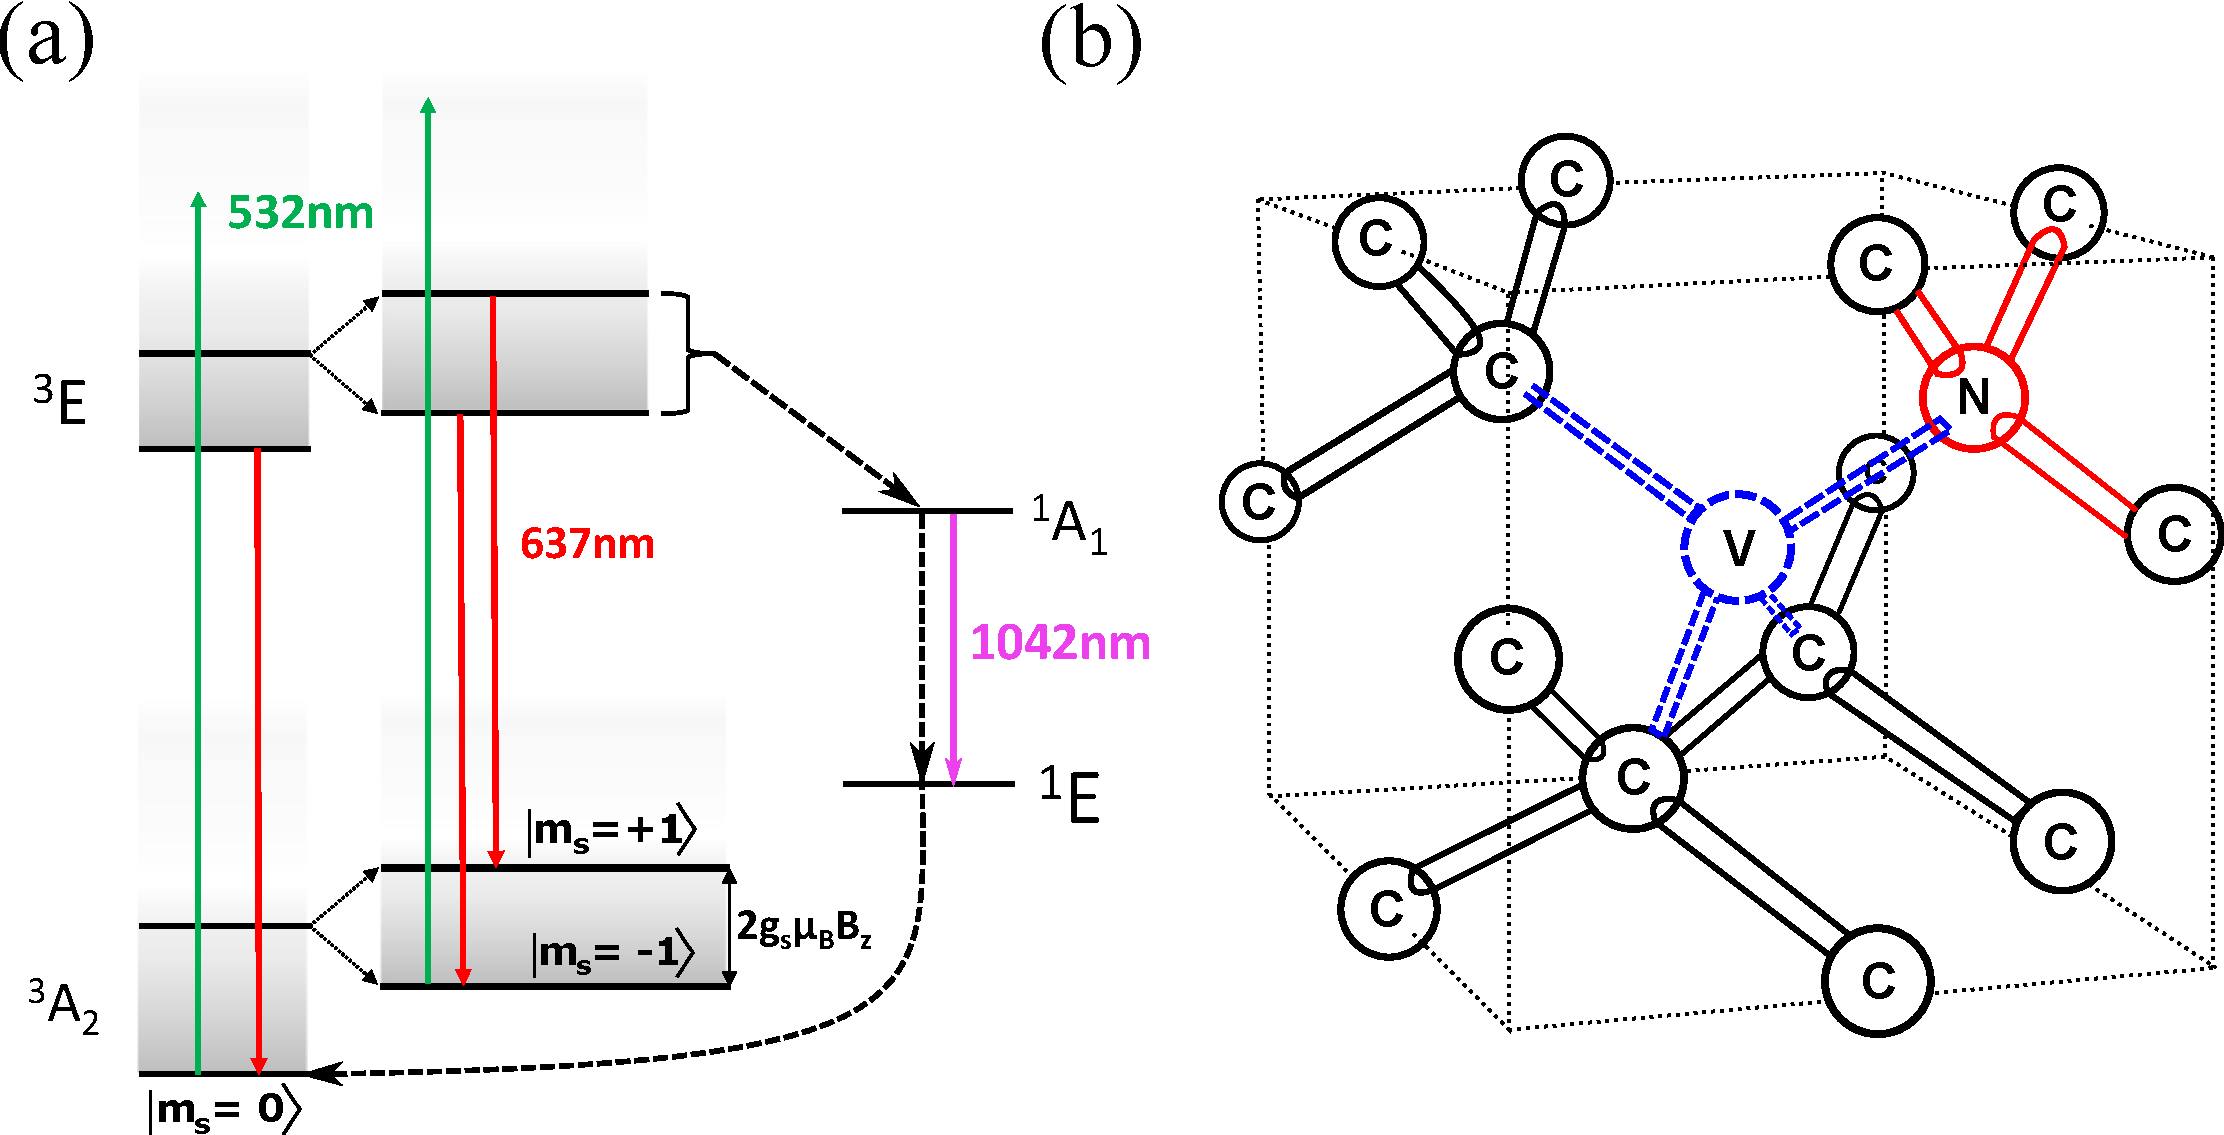
\includegraphics[width =\textwidth]{Intro_Fig_1.pdf}  
\caption{\textbf{The NV center} \textbf{a)} The NV level structure \textbf{b)} One of four crystal orientations of the NV.}
\label{Fig_one}
\end{figure}

\section{NV magnetometry} %This section needs work

Application of a static biasing magnetic field B\textsubscript{0} splits the $\ket{m_s = \pm1}$ levels via Zeeman interaction (equation \ref{hamiltonian}) proportional to the projection of the field onto the NV symmetry axis. When the NV is driven into one of these states and optically excited (generally achieved using 532nm CW or pulsed laser) it undergoes phononic-relaxation and settles into the corresponding sublevel of the excited state. These sublevels allow the NV to preferentially decay back down to the $\ket{0}$ ground state via an inter-system crossing and metastable state which are separated in the infrared. This non-spin-conserving process therefore provides the mechanism of spin polarizing the NV for continued MW driving. The NV spin state can then be read out by sweeping the driving microwave field and monitoring NV fluorescence in the visible band. A drop in fluorescence at a particular driving frequency indicates electron spin resonance (ESR) which can be monitored via lock-in amplification for any detuning due to a change in the external field\cite{jensen2017magnetometry,rondin2014magnetometry}. Since the NV can exist in one of four possible orientations---each orientation being equally likely---the ESR can be separated into eight distinct non-degenerate resonances which probe different field components. The various orientations act as basis vectors which collectively span the space and allow the total vector field to be reconstructed \cite{jensen2017magnetometry}. 

\subsection{Vector Magnetometry with NV Centers}\label{ch1:vect}

As mentioned in section \ref{sec:NVP}, the $C_{3v}$ symmetry of diamond allows NV centers to be aligned in four different orientations in the lattice. Since, at fields lower than 10 mT, the Zeeman splitting of the $\ket{\pm 1}$ is proportional to the vector field projection along the NV symmetry axis\footnote{At these low fields the terms in the NV Hamiltonian (see equation \ref{hamiltonian}) that are proportional to the perpendicular component of the field are suppressed to order $\sim B_{xy}^2 / D_{gs}$ and can therefore be neglected\cite{taylor2008high}} ($B_z$) the energy shifts can be determined by $\text{g}_\text{s} \upmu \text{b}\textbf{B} \cdot \textbf{\text{u}}_n,$ where $\textbf{\text{u}}_n$ ($n = 1,2,3,4$) is the unit vector along the n\textsuperscript{th} NV axis. By either sequentially or simultaneously measuring the Zeeman splitting between either the $\ket{0} \leftrightarrow \ket{+1}$ or $\ket{0} \leftrightarrow \ket{-1}$\footnote{The transition $\ket{-1} \leftrightarrow \ket{+1}$ can also be employed which yields the benefit that the energy shift becomes $2\text{g}_\text{s}\upmu_\text{b}\textbf{B}$ and therefore provides twice the signal over the other two transitions while simultaneously mitigating temperature effects \cite{neumann2013high}. However, this requires treatment of the full three-level spin system since the $\ket{-1} \leftrightarrow \ket{+1}$ splitting is a non-dipole allowed transition.} transitions of all four orientations, one can reconstruct the total vector field by generating the vector components ($B_x$, $B_y$, and $B_z$) from the projection along each of the crystallographic axes \cite{kitazawa2017vector,schloss2018simultaneous}.

\subsection{Continuous Wave Magnetometry}

For continuous wave magnetometry the ESR frequencies are continuously monitored (often using lock in amplification) since the external magnetic field is imprinted in their spectral positions $\omega_+$ and $\omega_-$ [Fig \ref{fig}]. As mentioned in section \ref{ch1:vect}, the four orientations of the NV in the diamond crystal lattice therefore result in eight distinct resonances when split by an external biasing field ($B_0$). Monitoring a minimum of three out of four resonances allows for the full vector reconstruction of the field. An infinitesimal additional magnetic field variation $\delta B$ shifts the resonances away from the known spectrum and the change in NV fluorescence, which is given by $\left(\frac{\partial \beta}{\partial B}\right) \cdot \delta B \cdot \tau$ \cite{rondin2014magnetometry}, is measured in the laboratory. The shot-noise limited sensitivity is then given as,
\begin{equation}
\eta_{cw} \approx \mathcal{P}_\mathcal{F}\frac{\hbar}{\text{g}_\text{s} \upmu_\text{B}} \frac{\Delta \omega \sqrt{\tau}}{C\sqrt{N \beta}}. 
\end{equation}
The signal contrast $C$ can be increased by driving the NV with stronger MW fields at the expense of power-broadening the linewidth $\Delta \omega$. However, the linewidth can be decreased down to a limit given the inhomogeneous dephasing time $T_2^*$ by reducing the laser and MW excitation strength \cite{dreau2011avoiding}, effectively decreasing the number of collected photons per measurement $\beta$. An optimization of contrast $C$, linewidth $\Delta \omega$, and collection $\beta$ yields an optimized sensitivity of \cite{pham2013magnetic}
\begin{equation}
\eta_{cw} \approx  \mathcal{P}_\mathcal{F}\frac{2\hbar}{\text{g}_\text{s} \upmu_\text{B}} \frac{1}{C\sqrt{N \beta T_2^*}}.
\end{equation}

%Talk about spin projection noise, photon shot noise, minimum detectable field \delta B, SNR etc.... see Scott and Chris's thesis

\subsection{Pulsed Ramsey-type Magnetometry} \label{Pulsed_Ramsey}

Strong microwave driving in a CW experiment broadens the ESR linewidth causing a reduction in magnetometer sensitivity. To take advantage of strong driving fields without incurring the effects of MW or pump laser power broadening, DC fields can be measured using a Ramsey pulse sequence. In this scheme microwave driving, spin polarization and sensing are all separated in time [Fig \ref{Fig_two}(a)]. After spin polarizing the NV electron spin into the $m_s = 0$ ground state, a resonant microwave pulse of length $\pi/2$ creates a superposition of the $\ket{0}$ and $\ket{+1}$ energy levels,
$$\ket{\Psi} = \frac{1}{\sqrt{2}}(\ket{0} + e^{i\phi}\ket{1}),$$
where the accumulated phase after precession time $\tau$ is $\phi = 2\pi \gamma B \tau$ where $B$ is the amplitude of the magnetic field to be determined and $\gamma = \text{g}_\text{s} \upmu_\text{B} / h = 2.8$ MHz/gauss the NV electron spin gyromagnetic ratio. Following the precession interval, a second $\pi/2$ MW pulse projects the spin back onto the quantization axis which is measured in the laboratory as a population difference between $\ket{0}$ and $\ket{+1}$, and read out optically through the spin dependent fluorescence of the NV center. Sensitivity is therefore improved by increasing the free precession time $\tau$ in order to maximize the accumulated phase, however, dipolar coupling to other magnetic impurities in the spin bath randomizes the accumulated phase after time $T_2^*$, the inhomogeneous NV dephasing time. Sensitivity in this scheme is optimized when the NV is allowed to precess in the magnetic field for $\tau \sim T_2^*$ and is given by 

$$\eta_{ramsey} \sim \frac{\hbar}{\text{g}_\text{s} \upmu_{\text{B}}} \frac{1}{C\sqrt{N \beta T_2^*}}.$$ 

\begin{figure}[t!]
\centering
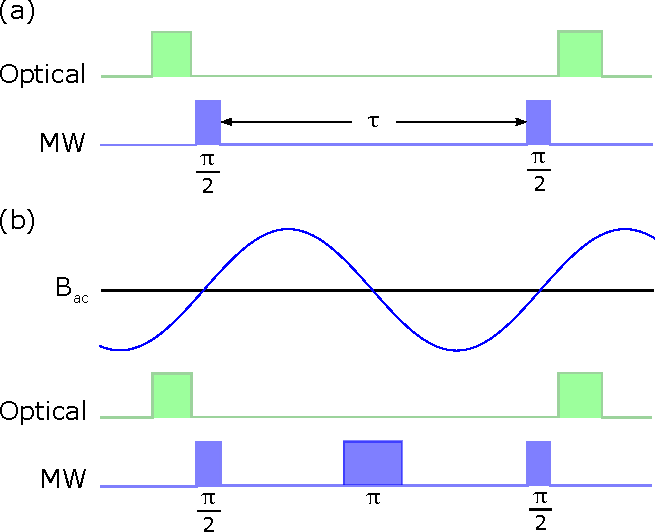
\includegraphics[scale = 0.9]{Ramsey_DC_AC.pdf}  
\caption{\textbf{Pulsed Magnetometry Sequences} \textbf{a)} Ramsey Sequence for DC magnetometry \textbf{b)} Hahn-Echo Sequence for AC magnetometry.}
\label{Fig_two}
\end{figure}

For AC magnetometry, the Ramsey sequence can be modified by bisecting the free precession interval $\tau$ with a single resonant $\pi$ pulse. The pulse is precisely timed to occur at the node of the oscillating field [Fig \ref{Fig_two}(b)] and deems to swap the accumulated phase from the $\ket{1}$ to the $\ket{0}$ state. For slow components of the external magnetic noise, the swap allows the second half of the free precession interval to compensate for phase randomization acquired during the first half of the interval. Using this sequence, $\tau$ can be increased to the homogeneous spin coherence time $T_2$ often orders of magnitude longer than $T_2^*$. The sensitivity for sensing an AC field is then improved when compared to sensing a DC field by a factor $\sqrt{T_2^*/T_2}$. This sequence is known as a Hahn-Echo sequence but AC magnetometry can be performed by more complex dynamical decoupling techniques \cite{carr1954effects, meiboom1958modified}.


\section{Rabi oscillations} \label{Rabi}

When an on- or near-resonant MW pulse is applied to a ground state transition in the NV, e.g. $\ket{0} \rightarrow \ket{+1}$, the NV spin state population will oscillate coherently between these two levels at a rate called the Rabi frequency ($\Omega_R$). This rate of oscillation is a function of the amplitude of the applied MW pulse. It is commonly measured by consecutively applying a polarizing laser pulse, a MW pulse, and a readout pulse [Fig. \ref{Fig1_3} (a)] and varying the MW pulse length after each iteration. 

\begin{figure}[t!]
\centering
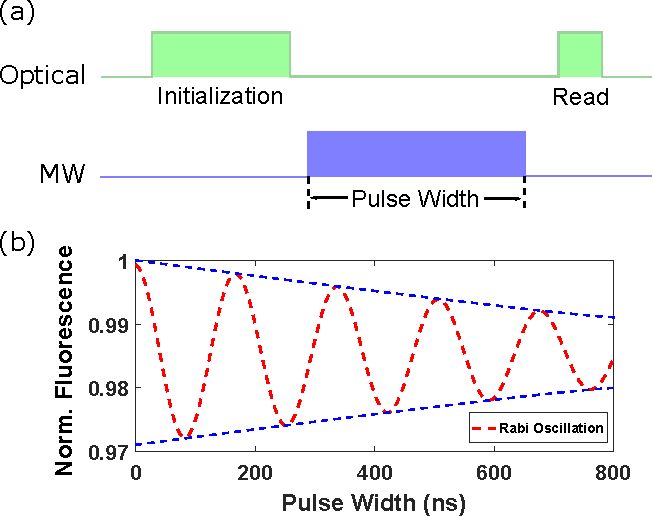
\includegraphics[scale = 0.9]{Rabi_sequence_and_figure.pdf}  
\caption{\textbf{Rabi pulse sequence and oscillations} \textbf{a)} Pulse sequence for detecting Rabi oscillation between two spin sublevels \textbf{b)} Example Rabi oscillations (\textcolor{red}{-- --}) with exponential decay envelope (\textcolor{blue}{ -- --}).}
\label{Fig1_3}
\end{figure}

Fig. \ref{Fig1_3} (b) plots a typical Rabi curve and its decay envelope. If the NV is originally in $\ket{0}$ (ie. at time $t = 0$) and we let the system evolve, then the probability that the spin is found in $\ket{+1}$ is $P_{+1} = \left(\frac{\omega_1}{\Omega_R}\right)^2 sin^2\left(\frac{\Omega_R t}{2}\right)$ where $\Omega_R = \sqrt{(\omega-\omega_0)^2-\omega_1^2}$ is the Rabi frequency, $\omega$ is the radial frequency of the oscillating field $B_1(\omega)$, $\omega_0$ the resonant frequency of the transition, and $\omega_1$ the (max) Rabi frequency at zero detuning. At resonance, the driving frequency is $\omega = \omega_0$ and the transition probability becomes $P_{+1} = sin^2\left(\frac{\omega_1 t}{2}\right)$. In order to therefore drive the entire population from e. g. $\ket{0}$ to $\ket{+1}$ as needed in, for example, the Hahn-Echo sequence described in \ref{Pulsed_Ramsey}, one needs to apply a pulse length such that $sin^2 \left(\frac{\omega_1 t}{2}\right) = 1$ which is satisfied when $t = \frac{pi}{\omega_1}$. For a Ramsey-type sequence that requires an equal superposition between $\ket{0}$ and $\ket{+1}$ one needs to apply half the $\pi$ pulse, $t = \frac{\pi}{2\omega_1}$. The Rabi oscillations however decay due to inhomogeneous broadening of the ensembles linewidth, and are therefore fit by the decaying envelope $\text{exp}\{-\left(PW/T\right)^p\}$, where PW is the pulse width and $T$ and $p$ are fit parameters.

\section{NV-MW coupling}

calculate coupling between NV center and MW photons in cavity.
